% !TeX spellcheck = da_DK
I forbindelse med kortlægningen af et område skal robotten have at vide hvor den er og hvordan den står i forhold til dens omgivelser.
I dette kapitel vil der blive beskrevet den valgte metode i forhold til lokalisering, ved brug af Microsoft Kinect og color-tracking.

 \section{Microsoft Kinect}\label{kinect}
En Kinect er et Natural User Interface (NUI) udviklet til Microsofts spillekonsol, Xbox.
Dens primære formål er at gøre det muligt at interagere med sin konsol vha. bevægelse og talte kommandoer.
Dog har den også mange andre anvendelsesområder, fx.:
%Den første version der udkom i november 2010~\cite{kinectWiki} er oprindeligt udviklet med henblik på at lokke nye typer brugere til Xbox med det argument at det via naturlig (og aktiv) bevægelse er sjovere og mere virkelighedstro at spille.
%
%I februar 2012 blev der lanceret en ny type Kinect, kaldet Kinect for Windows, der sammen med et Software Development Kit (SDK), der gør det muligt at udvikle både kommercielle og non-kommercielle applikationer til Kinect der kan køres på Windows platformen.
%Kort fortalt er Microsoft's Kinect mere end en input enhed gamere kan bruge for at gøre deres spiloplevelse mere virkelighedstro; af andre anvendelser kan f.eks. nævnes~\cite[s.~17]{kinectProgrammingGuide}:

\begin{itemize}
\item Optagelse af video i real-tid
\item Generere et dybde billede ved brug af kameraet og de to IR sensorer
\item Vurdering af omgivelserne ved hjælp af lyd
\end{itemize}

Oprindeligt eksisterede der kun en Kinect til XBox, men i februar 2012 blev der lanceret en ny type, kaldet Kinect for Windows, der sammen med et Software Development Kit (SDK), gør det muligt at udvikle både kommercielle og ikke-kommercielle applikationer til Windows platformen.

I dette projekt skal Kinecten benyttes til at bestemme robottens placering i ukendte omgivelser. 
Følgende afsnit giver en kort introduktion til Kinectens egenskaber.\cite{kinectProgrammingGuide}

\subsection{Opbygning af Kinect}\label{kinect:komponenter}
I denne rapport er det versionen Kinect for Windows der fokuseres på, da den giver bedst kompatibilitet med PC, samt det faktum at den er tilgængelig gennem universitetet.

%Dog kan det nævnes at forskellene mellem den og versionen til Xbox er meget små.
%Hardware mæssigt har Kinect for Windows den fordel at firmwaren indeholder en såkaldt Near Mode, hvilket gør det muligt at følge objekter indtil 40 cm fra enheden.
%Kinect for Xbox har ikke denne funktionalitet, og kan derfor kun følge objekter indtil 80 cm fra enheden, hvilket kan blive et problem i situationer hvor man ønsker at detektere små afstande via dybdebilleder.
%Kinect for Windows kan desuden også benyttes til kommercielle applikationer, hvor dens pendant er beregnet til hobbyister, generel udvikling og forskning~\cite[s.~16]{kinectProgrammingGuide}.
%
%For at Kinecten kan følge et objekt er Kinecten udstyret med et antal sensorer der nu vil blive beskrevet.

\begin{figure}
\centering
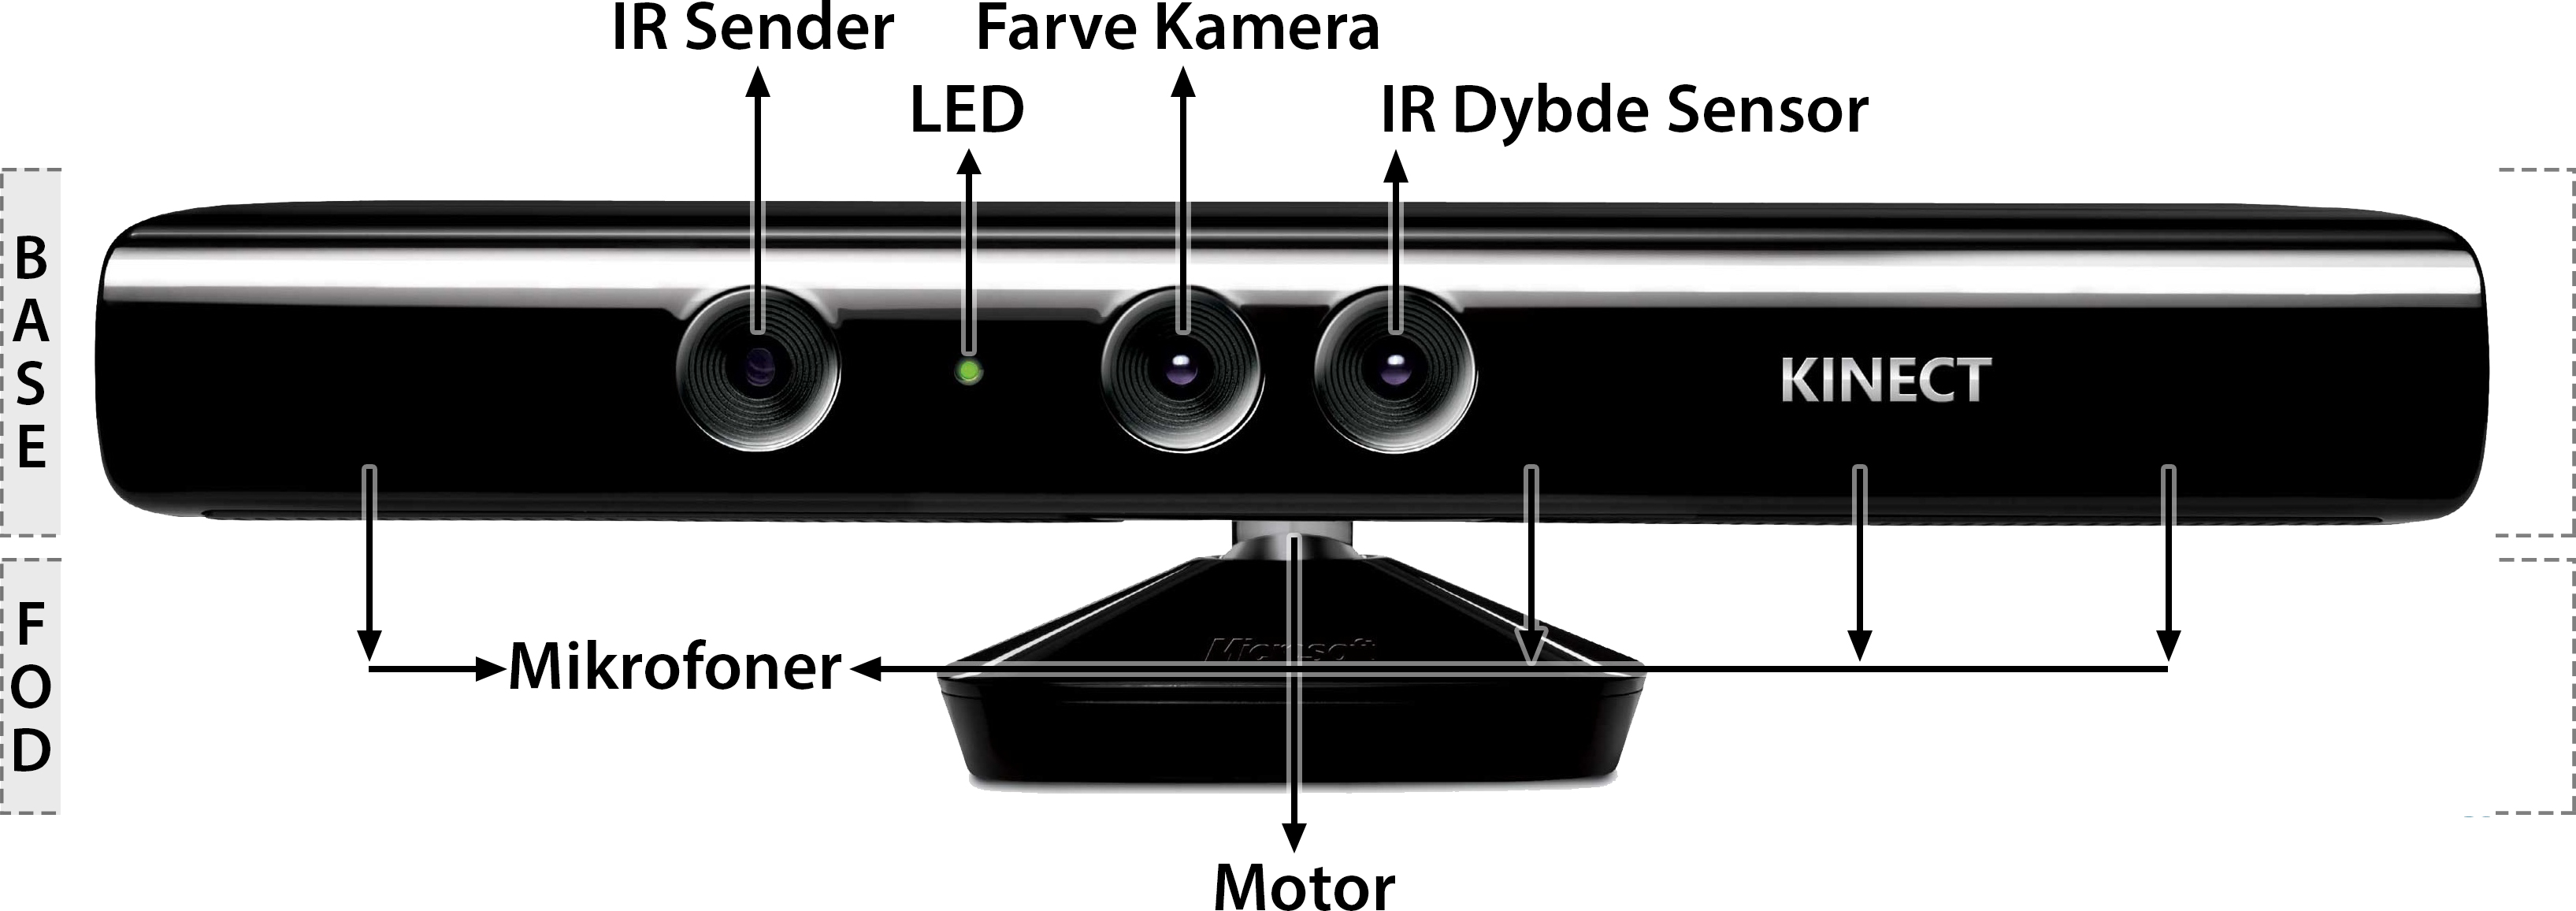
\includegraphics[width=1.0\textwidth]{kinect/kinect}
\caption{Microsoft Kinect for Windows.}
\label{kinect:opbygning}
\end{figure}

Microsoft Kinect for Windows består af en nogle hardware-komponenter, som kan tilgås via det medfølgende SDK\footnote{Der findes også andre tredjeparts SDK'er til Microsoft Kinect, men som ikke er relevante ift. projektet, hvorfor de ikke nævnes.}.
Microsoft Kinect for Windows består af følgende komponenter:

\begin{itemize}
\item Farvekamera
\item Infrarød (IR) sender
\item IR dybde sensor
\item Mikrofoner
\item Motor til justering af vinklen
\item LED
\item Accelerometer
\end{itemize}

Microsoft Kinect for Windows kan ses på \cref{kinect:opbygning}, sammen med dens synlige komponenter, som nævnes ovenfor.

For at løse lokaliseringsproblemet benyttes Kinectens farvekamera, der ses således bort fra alle dens andre komponenter.
Derfor bliver farvekameraets specifikationer på Kinecten i følgende afsnit beskrevet detaljeret.

\subsection{Farvekamera}\label{kinect:farvekamera}
For at gøre Kinecten i stand til at se, er den udstyret med et farvekamera, som er placeret ca. i midten af enheden (se evt. \cref{kinect:opbygning}).
Videoen bliver sendt som en RGB videostrøm, med mulighed for en opløsning på 1280x960 med en opdateringshastighed på 12 billeder i sekundet, eller en lavere opløsning på 640x480 og 30 billeder i sekundet.\cite{kinectForWindowsFeatures}
Kinecten har en horisontal betragtningsvinkel på 57\degree~og en vertikal betragtningsvinkel på 43\degree.
Et billede af Kinectens betragtningsvinkler kan ses på \cref{kinect:vinkler}.

\begin{figure}
\centering
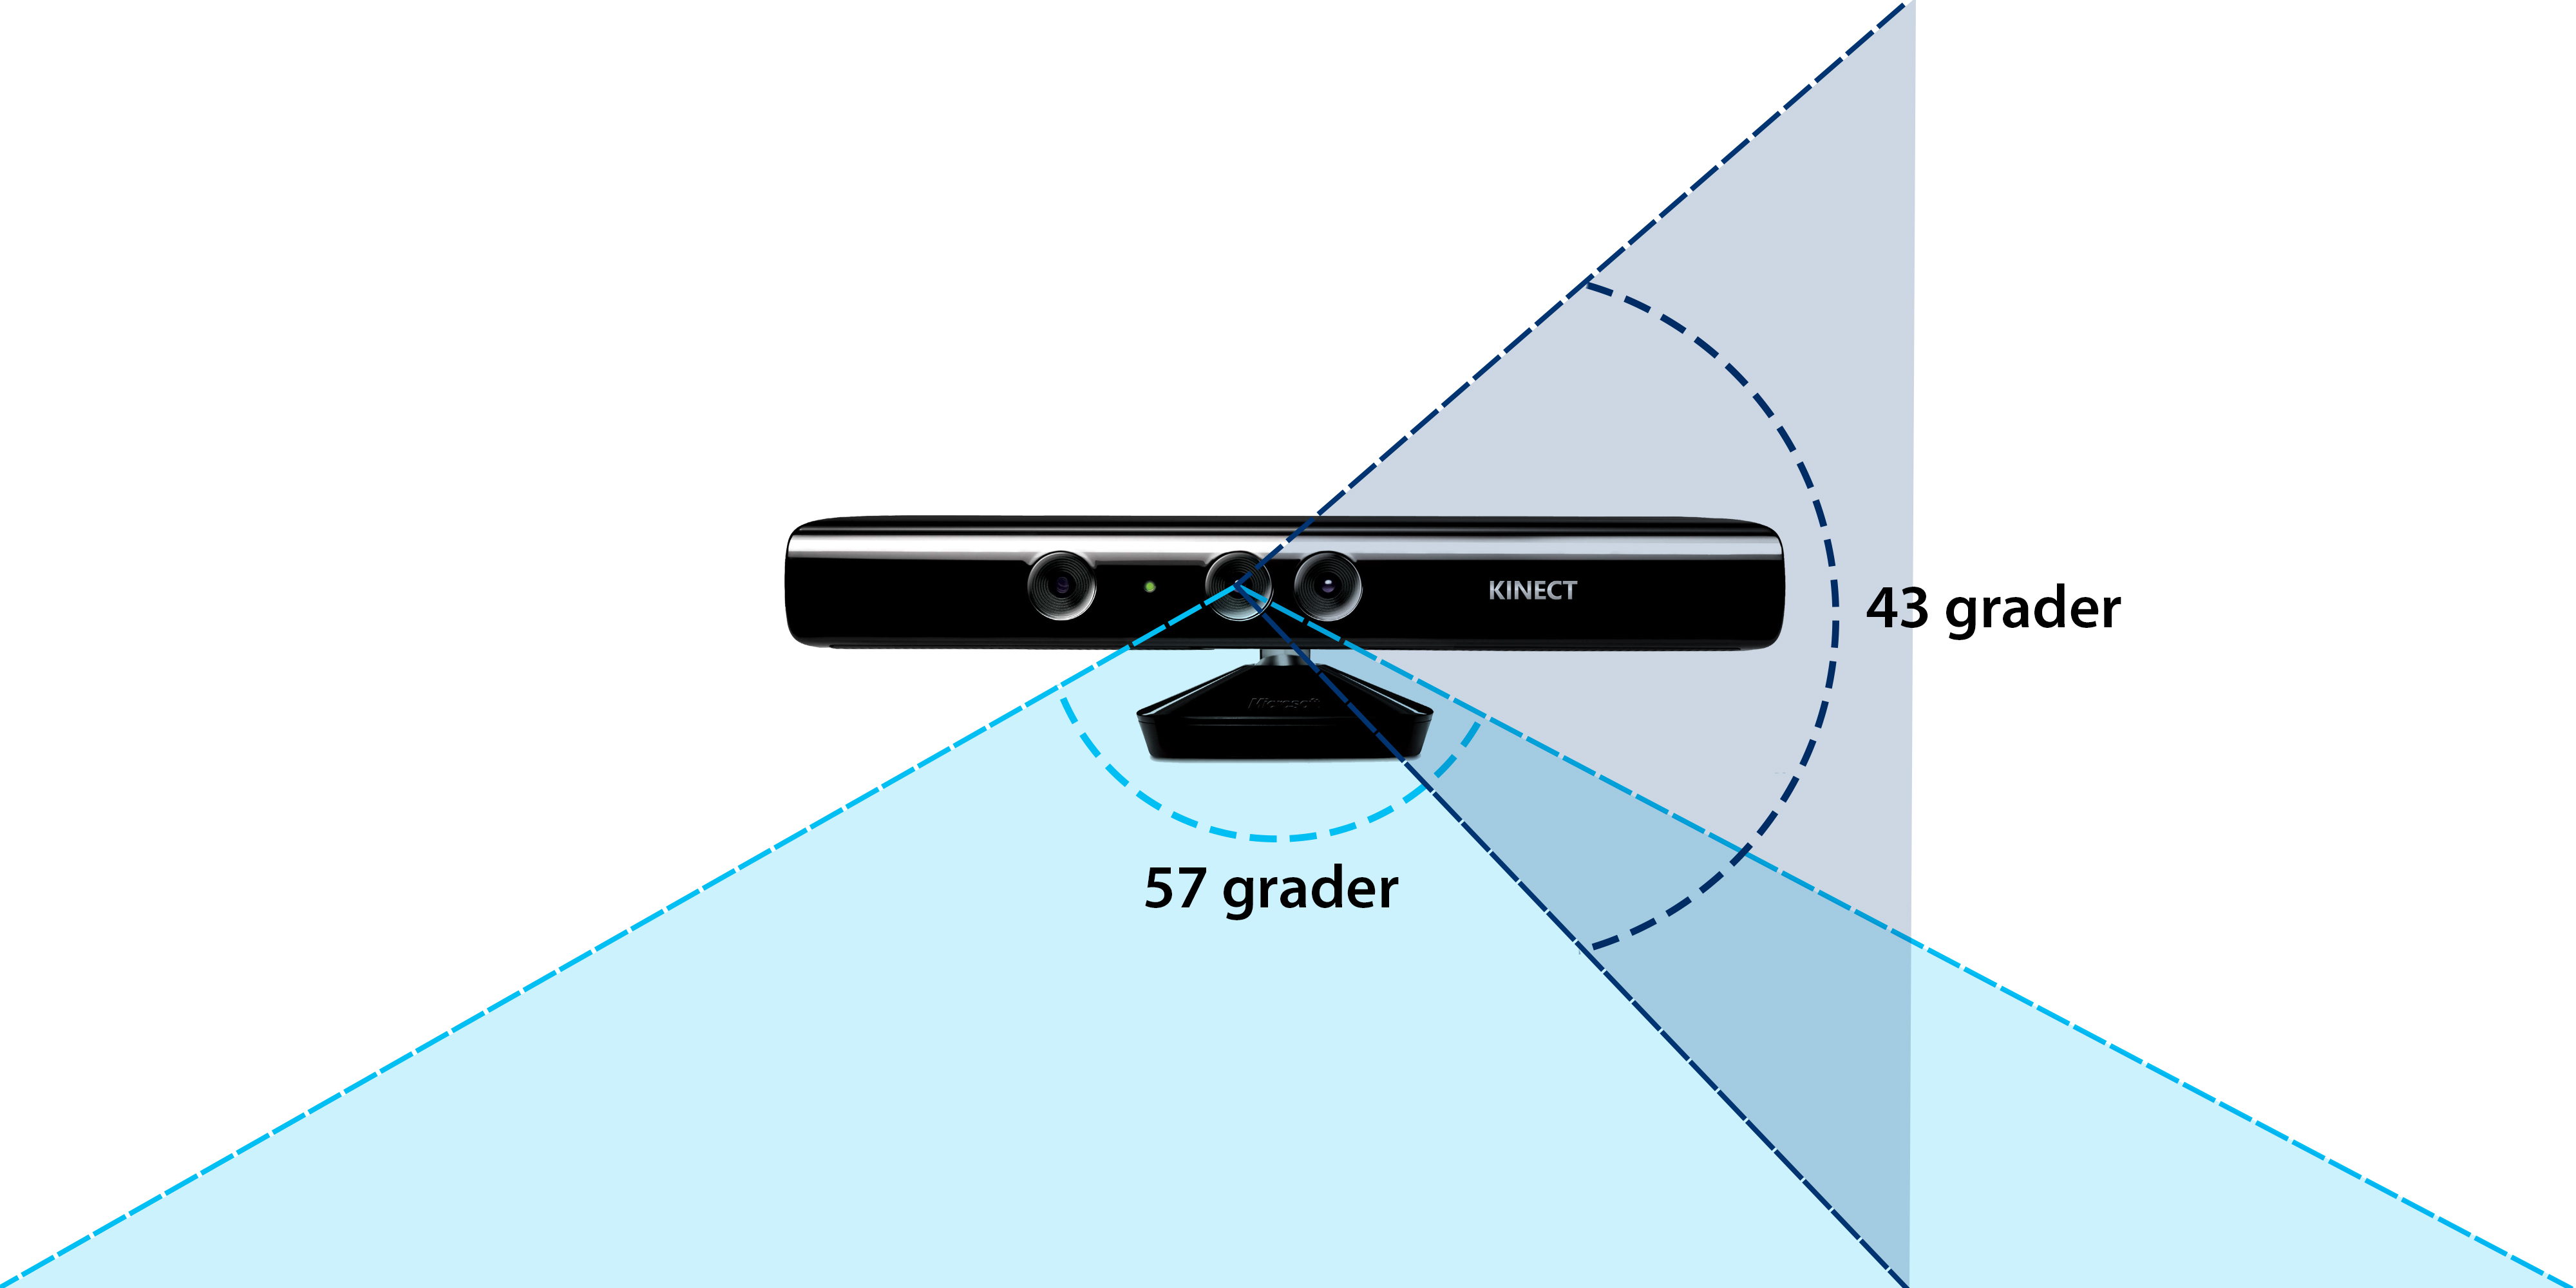
\includegraphics[width=1.0\textwidth]{kinect/kinect_view_angles}
\caption{Horisontale- og vertikale betragtningsvinkler for farvekameraet.}
\label{kinect:vinkler}
\end{figure}

\subsection{Valg af Kinect}\label{kinect:argumentation}
Microsoft Kinect giver generelt mange muligheder pga. alle dens komponenter, samt brugervenligheden overfor udviklere.
For at opsummere, så ser vi Kinectens overordnede fordele som:

\begin{itemize}
\item Nem montering
\item Nem tilslutning til PC
\item Mange sensorer
\item Gode udviklingsværktøjer
\item Tilgængelig gennem universitetet
\end{itemize}


Ovenstående fordele giver mange muligheder i forhold til hvordan Kinecten kan benyttes, men da der stræbes efter en simpel og pålidelig metode, vil dette smitte af på den endelige løsning.

\section{Kinect for Windows SDK}
Til Kinecten findes der et officielt SDK\footnote{ Version 1.8, udgivet 17 september, 2013~\cite{kinectSDK18}}, som åbner op for al funktionalitet i Kinecten med support fra Microsoft.

API'en er bygget op omkring en solid forståelse for menneskers bevægelser og karaktertræk, således API'en kan fungere som et interface, der kan genkende personers bevægelser, følge ansigter, genkende gestus og tale.
%Med Microsoft Kinect Toolkit installeret kan man endvidere få adgang til Kinect Fusion der gør det muligt at rekonstruere 3D objekter ud fra Kinectens kamera og dybdebilleder fra IR sensorerne.~\cite{kinectForWindowsFeatures}

\subsection{Kinect API}\label{kinect:kinectapi}
De følgende afsnit vil fokusere på, hvordan SDK'et benyttes for at tilgå Kinectens mest basale funktionalitet, med fokus på hvordan billeddata hentes fra dets farvekamera.

\subsubsection{Initialisering}
Før Kinecten kan anvendes og der er adgang til dens sensorer, skal Kinecten initialiseres.
Et eksempel på initialisering af en Kinect kan se i \cref{kinect:initialisering}. \lstinline[style=csharp]|Form1_Load| metoden i \cref{kinect:load} køres ved applikationens opstart og sørger for at starte sensoren, hvis den findes. Fra \cref{kinect:enablebegin} til \cref{kinect:enableend} tændes for de billedstreams, der er nødvendige. I eksemplet tændes for RGB-kameraet, dybdekameraet, samt skeletdetektoren. Hvis der ikke er en Kinect tilsluttet, meldes der fejl (\cref{kinect:error}).

\begin{lstlisting}[style=csharp, label=kinect:initialisering, caption={Initialisering af en Kinect sensor.}]
KinectSensor sensor;

private void Window_Loaded(object sender,
	RoutedEventArgs e) (*\label{kinect:load}*)
{
    if (KinectSensor.KinectSensors.Count > 0)
    {
        this.sensor = KinectSensor.KinectSensors[0];
        StartSensors();
        
        this.sensor.ColorStream.Enable();(*\label{kinect:enablebegin}*)    
	this.sensor.DepthStream.Enable();
        this.sensor.SkeletonStream.Enable();(*\label{kinect:enableend}*)
	this.sensor.ColorFrameReady += 
		sensor_ColorFrameReady; (*\label{kinect:event}*)
    }

    else
    {
        MessageBox.Show("No Kinect connected"); (*\label{kinect:error}*)
        this.Close();
    }

}

private void StartSensors()
{
    if (this.sensor != null && !this.sensor.IsRunning)
    {
        this.sensor.Start();
    }
}
\end{lstlisting}

\subsubsection{Visning af Kinectens billeddata}
For at vise de billeder, som Kinecten optager, benyttes \lstinline[style=csharp]!sensor_ColorFrameReady! eventet. 
Dette event affyres hver gang der modtages et nyt billede fra Kinecten. 
Et eksempel på visning af Kinectens data ses i \cref{kinect:picture}, hvor der i \cref{kinect:openframe} gemmes en reference til den frame, der netop er blevet optaget af Kinecten.
I \cref{kinect:pixeldata} kopieres data over i et bytearray for at arbejde på dataen. 
I \cref{kinect:source} sættes billedets source til et billede konstrueret ud fra dataen fra Kinecten.
Billedet \lstinline[style=csharp]|imageFrame| viser nu hvad Kinecten ser.

\begin{lstlisting}[style=csharp,caption={Visning af billeddata fra Kinectens RGB-kamera.}, label=kinect:picture]
byte[] pixelData = null;
void sensor_ColorFrameReady(object sender,
	ColorImageFrameReadyEventArgs e)
{
    using (ColorImageFrame imageFrame = 
    	e.OpenColorImageFrame()) (*\label{kinect:openframe}*)
    {
        if (imageFrame == null)
            return;

            this.pixelData = 
            	new byte[imageFrame.PixelDataLength];(*\label{kinect:pixeldata}*)

            imageFrame.CopyPixelDataTo(this.pixelData);

            int stride = imageFrame.Width *
            	imageFrame.BytesPerPixel;

            this.KinectImage.Source = 
            	BitmapSource.Create(
            imageFrame.Width, imageFrame.Height, 
            	96, 96, PixelFormats.Bgr32, null, 
            		pixelData, stride); (*\label{kinect:source}*)
    }
}    
\end{lstlisting}

\section{Colortracking}
Til at lokalisere robotten er det valgt at benytte Kinectens kamera og en farvegenkendelsesalgoritme.
På den måde er det muligt at finde robotten i billedet uden at være afhængig af en bestemt form eller konstruktion.
Derimod skal der bare være mulighed for at sætte nogle farvede mærkater på robotten.
Ideen er at sætte to forskelligt farvede mærkater på kroppen af robotten og følge dem hver for sig. 
Dette vil da give en mulighed for at beregne midtpunktet af disse to mærkater samt robottens vinkel, hvilket svarer til robottens positur.